\documentclass[
    12pt,                               % Schriftgröße
    DIV=14,                     % Satzspiegel
    %BCOR=10mm,                 % Bindekorrektur
    parskip=half+,              % + - * Absatzeinrückung 
    bigheadings,                % Große Überschriften
    cleardoubleempty,   % Keine Kopfzeile bei neuer 
    halfparskip,                % Halbe Zeile Abstand bei neuem Absatz
    %openright                  % Neues Kapitel bei Doppelseitigem Layout rechts
    ]{scrreprt} % 

\usepackage[T1]{fontenc}
\usepackage[utf8]{inputenc}
\usepackage[table,dvipsnames]{xcolor}
\usepackage{lmodern}
\usepackage{listings}
\usepackage{subcaption}
\usepackage{tikz}
\usepackage{float}
\usepackage{amsmath}
\usepackage{hyperref}

\hypersetup{
    unicode=true,    % allow unicode chars in hyperlinks
    breaklinks=true,
    hidelinks,       % disable frames around links
    colorlinks=true, % show links in a different color
    linkcolor=%
        black,       % use a black color for links
    urlcolor=%
        Blue,    % use a dark blue color for file references
    citecolor=%
        OliveGreen,   % use a dark green color for cite notes
    % the following is additional stuff
    pdftitle=Component Identification in Firmware Images,       % title of the PDF
    pdfauthor=Jakob Loew,      % author of the PDF
    pdfkeywords=security graphs call graphs graph matching edit distance,    % keywords of the PDF
    pdfcreator=Jakob Loew,     % creator of the PDF
    pdfproducer=Jakob Loew,    % producer of the PDF
}

\usetikzlibrary{calc,arrows,positioning}
\tikzset{
    %define standard arrow tip
    >=stealth',
    %define arrow style
    pil/.style={
           ->,
           thick,
           shorten <=4pt,
           shorten >=4pt,}
}

% Set language to english
%\usepackage[english]{babel}

\titlehead{
  \hfil
  \includegraphics[width=0.5\textwidth]{thi_logo_cropped}
  \hfil
}

\title{Component Identification in Firmware Images}

\author{Jakob Löw}

\date{}

\publishers{
        \begin{tabular}{rl}
                \textbf{First corrector}        & Prof. Dr.-Ing. Hans-Joachim Hof \\
                \textbf{Technical Supervision}  & Dominik Bayerl \\
                \textbf{Date of filing}         & 04.05.2020 \\
        \end{tabular}
}

\begin{document}

\maketitle
\newpage

\tableofcontents
\newpage

\chapter{Abstract}
In the past finding known functions in binaries was often solved using code signatures. For example antivirus programs generate checksums of machine code in order to find malicious code segments. Or when injecting code into a running program often a known function is searched using a machine code pattern, then the function is hooked by overwriting its first instruction by a jump to custom code. \\
Both these approaches fail when the target code changes slightly. Apart from code changes this can also happen when using a different compiler or other compilation options. While updating the code checksum or pattern fixes that problem this paper aims at developing an algorithm which can still identify libraries in binaries even when their machine code is not identical. \\
The goal of this paper is to create an algorithm which given two binary files, usually a library and a linked executable, can determine if the library is included in the executable. In reality most executables for desktop operating systems use dynamic linking, in which case it is trivial to tell what libraries are used by the program. For firmware files used in microprocessors however all libraries are statically linked and thus included in the firmware file. Furthermore these libraries are often compiled with options specific to the use case, functions are left out or are otherwise optimized. This results in the library footprint in the firmware to hardly ever be identical to a binary obtained by compiling the binary in a different context. \\
Instead of code signatures or patterns the approach presented in this paper is based on call graphs. In the first step a call graph $G_2$ is generated for the firmware and one $G_1$ for the library. In the second step an error tolerant subgraph matching algorithm calculates the minimal amount of changes required to $G_1$ in order to make $G_1$ a subgraph of $G_2$. By applying a reasonable threshold to this distance we can determine wether the library is included in the firmware. \\
Chapter \ref{chap:notation} covers the notation used in chapters \ref{chap:graphacquisition} and \ref{chap:graphmatching} which cover call graphs and graph matching respectively. Afterwords in chapter \ref{chap:libraryidentification} these steps are adapted and combined to match the library graph to the executable graph. In the last chapter \ref{chap:validation} we show the performance and accuracy of the described method by applying it to real world examples.

\chapter{Notation} \label{chap:notation}
This chapter summarizes the notations used in this paper when describing graphs. \\
A graph is denoted as $G$, these can be \textit{attributed} and/or \textit{directed}. They consist of $n$ nodes, also called vertices, denoted as $v_i$ for the $i$th node. Two nodes $v_a$ and $v_b$ can be connected using an edge denoted as $e_{ab}$ or $e_{ba}$. The total amount of edges connected to a node $v_i$ is called its \textit{degree} denoted as $deg(v_i)$. All nodes connected to a node $v_i$ are denoted as $L_i$ with $L_i = \{v_j \: | \: e_{ij} \in G\}$. \\
For directed graphs an edge $e_{ab}$ is an edge from $v_a$ to $v_b$, which is different from the edge $e_{ba}$ that connects from $v_b$ to $v_a$. Thus for directed graphs each node has an outgoing degree $deg_{\text{out}}(v_i)$ and an incoming degree $deg_{\text{in}}(v_i)$. Similarly each node $v_i$ has two sets of adjacent nodes: $L_{\text{out}_i}$ are the nodes connected via an outgoing edge, while $L_{\text{in}_i}$ are the nodes connected via an incoming edge. \\
Attributed graphs additionally have a labeling function $l(v_i)$ which returns the label of node $v_i$. In a more general form a $l(v_i)$ can return any type attribute and is not limited to labels. \\
The table in figure \ref{fig:notation} shows an overview of these notations. \\

\begin{figure}[H]
	\centering
	\begin{tabular}{l | l | l}
		$G_i$		& a graph $i$ & \\ \hline
		$v_i$		& the $i$th node in a graph \\ \hline
		$e_{ij}$	& an edge connecting nodes $v_i$ and $v_j$ \\ \hline
		$l(v_i)$	& a function returning the label of $v_i$ & \\ \hline
		$n$			& the number of nodes in a graph & $n = |G|$ \\ \hline
		$L_i$		& the set of nodes connected to $v_i$ & $L_i = \{v_j \: | \: e_{ij} \in G, e_{ji} \in G\}$ \\ \hline
		$L_{\text{in}_i}$ & the set of nodes connected via an incoming edge to $v_i$ & $L_{\text{in}_i} = \{v_j \: | \: e_{ji} \in G\}$ \\ \hline
		$L_{\text{out}_i}$ & the set of nodes connected via an outgoing edge to $v_i$ & $L_{\text{out}_i} = \{v_j \: | \: e_{ij} \in G\}$ \\ \hline
		$deg(v_i)$	& the amount of nodes connected to $v_i$ & $deg(v_i) = |L_i|$ \\ \hline
		$deg_{\text{in}}(v_i)$	& the amount of incoming nodes connected to $v_i$ & $deg_{\text{in}}(v_i) = |L_{\text{in}_i}|$ \\ \hline
		$deg_{\text{out}}(v_i)$	& the amount of outgoing nodes connected to $v_i$ & $deg_{\text{out}}(v_i) = |L_{\text{out}_i}|$ \\
	\end{tabular}
	\caption{Graph notation overview}
	\label{fig:notation}
\end{figure}

\chapter{Call graphs} \label{chap:graphacquisition}
A call graph describes the relations between functions in a program. Each node $v_i$ in the graph resembles one function in the program. Call graphs are usually \textit{directed graphs}. When a function $a$ contains a call to function $b$ an edge $e_{ab}$ is created in the call graph. When symbol information, i.e. function naming, is available, call graphs are \textit{attributed graphs}. In this case the labeling function $l(v_i)$ returns the name of function associated with node $v_i$. \\
In reality often symbols are stripped, making them unavailable and thus the call graph an \textit{unattributed graph}. \\
Figure \ref{fig:callgraph:example} shows the call graph to the example pseudo code in \ref{fig:callgraph:example:code}. \\
While call graphs can easily be created from source code, in practice the source code is unavailable. Only the compiled binary is supplied, thus the sections in this chapter will cover methods for retrieving a call graph from a binary.

\begin{figure}[H]
	\centering
	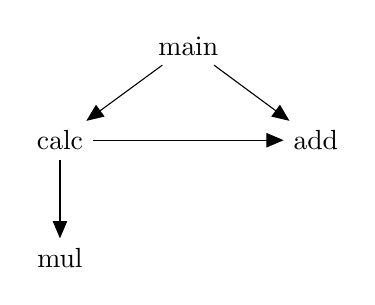
\begin{tikzpicture}[node distance=1cm, auto]
    	\node[draw=none] (main) {main};
    	\node[draw=none, below left=of main] (calc) {calc};
    	\node[draw=none, below right=of main] (add) {add};
    	\node[draw=none, below=of calc] (mul) {mul};
    	
    	\path [-{triangle 45}]
    		(main) edge (calc)
    		(main) edge (add)
    		(calc) edge (add)
    		(calc) edge (mul)
    	;
    \end{tikzpicture}
	\caption{Call graph of the code in figure \ref{fig:callgraph:example:code}}
	\label{fig:callgraph:example}
\end{figure}

\begin{figure}[H]
	\begin{lstlisting}[language=Python]
def main():
	return add(calc(), 5)
def calc():
	return add(mul(6, 5), 7)
def add(x, y):
	return x + y
def mul(x, y):
	return x * y
	\end{lstlisting}
	\caption{Pseudo code for demonstrating call graphs}
	\label{fig:callgraph:example:code}
\end{figure}

\section{Function prolog and epilog} \label{sec:funcprolog}
A simple approach at finding functions in a binary is searching for function prolog and epilogs. A classic function prolog consist of saving the base pointer to the stack, loading the new base pointer and decrementing the stack pointer. On the x64 architecture this commonly results in three instructions:
\begin{lstlisting}
pushq %rbp
movq %rsp, %rbp
subq $32, %rsp
\end{lstlisting}
At the end of the function stack and base pointers have to be restored. The x64 architecture has a special instruction \verb'leave' which first moves the value of \verb'%rbp' into \verb'%rsp' and then popping a value from the stack into \verb'%rbp'. Together with a \verb'ret' instruction this forms a common function epilog:
\begin{lstlisting}
leaveq
retq
\end{lstlisting}

Leaf\footnote{A leaf function does not call any other functions, it is thus a leaf in the call tree} functions often do not need to alter stack and base pointer. They place their local stack variables, if any, in the red zone\footnote{128 byte zone below the stack pointer which remains touched on interrupts} addressed relative to the unchanged stack pointer. Thus they have neither a prolog nor an epilog, making the prolog and epilog method unable to find such functions. \\
Furthermore this method finds only the nodes (i.e. the functions) of the call graph. There is no information on the edges of the graph retrieved.

\section{Call instruction based acquisition} \label{sec:graphfromcall}
In order to find the edges of the call graph the \verb'call' instructions have to be inspected. The following presents an algorithm which can not only derive the edges of the call graph, but also the nodes from \verb'call' instructions in a binary file.

Each \verb'call' instruction $I$ has a target address $T$ and a source address $S$ (i.e. the address of the call instruction in the binary). Each \verb'call' instruction resembles one directed edge in the call graph from $S'$ to $T$. The instructions source $S$ does not directly map to the source function $S'$, instead it lies somwhere \textit{in} the source function. $T$ however directly points to the start of the target function. The following example code illustrates this:
\begin{lstlisting}
0000000000001135 <foo>:
[...] 

000000000000114a <bar>:
    114a:	48 83 ec 08          	sub    $0x8,%rsp
    114e:	b8 00 00 00 00       	mov    $0x0,%eax
    1153:	e8 dd ff ff ff       	callq  1135 <foo>
    1158:	48 83 c4 08          	add    $0x8,%rsp
    115c:	c3                   	retq
\end{lstlisting}

The call instruction at location $S = 0x1153$ jumps to $T = 0x1135$. Thus we know there exists a function at address $0x1135$ and we know there exists an directed edge from $S'$ to $T$. In order to find $S'$ we have find the largest $T_j$ of a call instruction $J$ for which $T_j < S$ \\
By iterating over all call instructions in a binary once we can extract all functions. Afterwords we can use the list of functions to find the source functions of all \verb'call' instructions and can create an directed edge in the call graph.

\section{radare2} \label{sec:radare2}
\textit{Radare2} is an open source binary reverse engineering utility. It allows to analyze binaries using a text based user interface. Radare2 does not provide a direct API for programmatically analyzing binaries, instead there is a wrapper library called \textit{r2pipe} which allows sending commands as if they were typed into the user interface. Luckily there is already a command built in for dumping the call graph of a binary in JSON format. After calling \verb'aaa' for analyzing a loaded binary, the \verb'agCj' dumps the extracted call graph in json format.
% TODO moar!

\section{Call graph altering compiler optimizations} \label{sec:optimizationproblems}
There are a couple of compiler optimizations which interfere with some or all of the above mentions methods of call graph retrieval. The simplest of these optimization is the removal of classic function prologs and epilogs in leaf functions as already described in section \ref{sec:funcprolog}.

Another difficulty in finding functions are tail calls. When a function ends with a call and returns nothing or the result of that call, this is called a tail call. The following dummy C-code shows such a tail call:
\begin{lstlisting}[language=C]
int foo(int x)
{
	return x + 2;
}
int bar(int y)
{
	return foo(y + 3);
}
\end{lstlisting}

In these cases often the call to the function and the function epilog are replaced by a simple jump to the tail callee. When the tail callee returns it returns directly to the caller of the tail caller. Thus the above code sample is compiled to:
\begin{lstlisting}
foo:
  movl %edi, %eax
  addl $2, %eax
  ret
bar:
  addl $3, %edi
  jmp foo
\end{lstlisting}

The problem is that even though there is a jump from function \verb'foo' to \verb'bar' there is neither a call instruction nor a function prolog or epilog in \verb'foo' making the above methods unable the edge from $v_{bar}$ to $v_{foo}$.

%TODO: .o files fails (call instruction offsets), ...

\chapter{Graph matching} \label{chap:graphmatching}
Given two graphs $G_1$ and $G_2$ graph matching describes the process of mapping a node $v_1 \in G_1$ to a node $v_2 \in G_2$. \\
Graph isomophism, as described in the following section is an \textit{error-intolerant} approach at graph matching. In order for two graphs to be isomorph they have to be \textit{identical}. \\
Graph edit distance, as covered in sections \ref{sec:editdistance} to \ref{sec:beliefpropagation}, is a metric for measuring the distance between two graphs. It allows to make claims about the graph relations even when the graphs are isomorph. Is it thus an \textit{error-tolerant} approach to graph matching.

\section{Graph isomorphism}
Two graphs $G_1$ and $G_2$ are called isomorph when there exists a mapping $f(v_x) \rightarrow v_a$ with $v_x \in G_1$ and $v_a \in G_2$ if and only if $\forall v_x \in G_1: \; \{f(v_y) \: | \: v_y \in L_x\} == L_a$. \\
Or in words: Two graphs are called isomoph when there exists a mapping from nodes in $G_1$ to nodes in $G_2$ such that mapping all nodes connected to a node $v_x \in G_1$ returns the set of all nodes connected to $v_a \in G_2$ with $v_a$ being the node mapped to $v_x$. \\
Figure \ref{fig:isomorph:graph} shows a graph which is isomorph to the graph from figure \ref{fig:callgraph:example} with the mapping shown in figure \ref{fig:isomorph:mapping}.

\begin{figure}[H]
        \centering
        \begin{subfigure}[b]{0.45\textwidth}
                \centering
                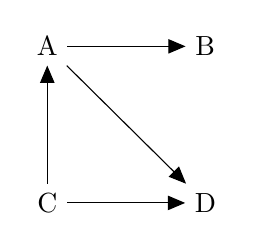
\begin{tikzpicture}[node distance=1.5cm, auto]
					\node[draw=none] (main) {C};
					\node[draw=none, above=of main] (calc) {A};
					\node[draw=none, right=of main] (add) {D};
					\node[draw=none, right=of calc] (mul) {B};
			
					\path [-{triangle 45}]
						(main) edge (calc)
						(main) edge (add)
						(calc) edge (add)
						(calc) edge (mul)
					;
                \end{tikzpicture}
                \caption{A graph isomorph to figure \ref{fig:callgraph:example}}
                \label{fig:isomorph:graph}
        \end{subfigure}
        ~
        \begin{subfigure}[b]{0.45\textwidth}
                \centering
				\begin{tabular}{c | c}
					$v_i \in G_{\text{\ref{fig:isomorph:graph}}}$ & $f(v_i) \in G_{\text{\ref{fig:callgraph:example}}}$ \\
					\hline
					A & calc \\
					B & mul \\
					C & main \\
					D & add \\
				\end{tabular}
                \caption{Mapping of nodes in figure \ref{fig:isomorph:graph} to nodes in figure \ref{fig:callgraph:example}}
                \label{fig:isomorph:mapping}
        \end{subfigure}

        \caption{Simple graph isomorphism example}
        \label{fig:isomorph}
\end{figure}

% TODO: subgraph isomorphism

\section{Graph edit distance} \label{sec:editdistance}
In our case a graph isomorphism algorithm is not enough. The callgraph of a library embedded in an executable often is not fully isomorph to the orginal call graph taken from the libraries object files. This can be caused by compiler optimizations, the linker removing unused functions or even different library configurations. \\
Thus instead of full graph isomorphism we need to calculate a the \textit{graph edit distance} between two graphs $G_a$ and $G_b$. This distance describes how many nodes or edges have to be changed, added or removed in order to make $G_a$ a subgraph of $G_b$. Figures \ref{fig:graphmatch:example:a} and \ref{fig:graphmatch:example:b} show two simple graphs, which have an edit distance of $4$. Or in other words: Four changes have to be made in order to turn \ref{fig:graphmatch:example:a} into \ref{fig:graphmatch:example:b}, removing the edges $e_{CD}$ and $e_{BD}$, removing the node $v_D$ and adding the edge $e_{BC}$. \\

%TODO edit operations

\begin{figure}[H]
        \centering
        \begin{subfigure}[b]{0.45\textwidth}
                \centering
                \begin{tikzpicture}[node distance=2cm, auto]
                	\node[draw=none] (A) {A};
                	\node[draw=none, below left=of A] (B) {B};
                	\node[draw=none, below right=of A] (C) {C};
                	\node[draw=none, right=of B, xshift=-0.5cm] (D) {D};
                	
                	\path [-]
                		(A) edge (B)
                		(A) edge (C)
                		(C) edge (D)
                		(D) edge (B)
                	;
                \end{tikzpicture}
                \caption{}
                \label{fig:graphmatch:example:a}
        \end{subfigure}
        ~
        \begin{subfigure}[b]{0.45\textwidth}
                \centering
                \begin{tikzpicture}[node distance=2cm, auto]
                	\node[draw=none] (A) {A};
                	\node[draw=none, below left=of A] (B) {B};
                	\node[draw=none, below right=of A] (C) {C};
                	
                	\path [-]
                		(A) edge (B)
                		(A) edge (C)
                		(C) edge (B)
                	;
                \end{tikzpicture}
                \caption{}
                \label{fig:graphmatch:example:b}
        \end{subfigure}

        \caption{Simple graph edit distance example}
        \label{fig:graphmatch:example}
\end{figure}

As shown by \cite{compstars} calculating the graph edit distance is a NP-Complete problem.
The following sections will cover various approaches and algorithms for calculating the edit distance of two graphs.

%\section{Exact edit distance}
%TODO % https://www.researchgate.net/publication/275463562_An_Exact_Graph_Edit_Distance_Algorithm_for_Solving_Pattern_Recognition_Problems

\section{Approximating graph edit distance} \label{sec:approxeditdistance}
In order to reduce the complexity of calculating the graph edit distance various efficient algorithms have been suggested. They usually compare a local structure around two nodes $v_1 \in G_1$ and $v_2 \in G_2$. The most common local structures are just the node, the node and its edges (i.e. its degree) and the star structure\cite{commoncost1, commoncost2}. \\
Defining the cost on the node requires a labeled graph and works by comparing node labels denoted as $l(v_i)$:
\begin{equation}
	\lambda_{\text{node}}(v_1, v_2) = \begin{cases}
		0 & \text{if } l(v_1) = l(v_2) \\
		1 & \text{otherwise}
	\end{cases}
\end{equation}

A degree based cost function additionally considers a nodes degree denoted as $deg(v)$, i.e. the amount of edges connected to node $v$:
\begin{equation}
	\lambda_{\text{edge}}(v_1, v_2) = \lambda_{\text{node}}(v_1, v_2) + |\text{deg}(v_1) - \text{deg}(v_2)|
\end{equation}

Star based cost functions use the node, its edges and the nodes connected to these edges. In generally a star structure of a node $v_i$ has the form $(v_i, L, l)$, where $L$ is the set of nodes directly connected to $v_i$. $l$ is the label function. Additionally this cost function uses the multiset of labels in $L$ denoted as $\Psi$. This multiset can then be used to define the minimum node distance $M(L_1, L_2)$ between two set of nodes $L_1$ and $L_2$. The star cost function is defined as\cite{compstars}:

\begin{equation}
	\Psi_i = \{ l(v_j) \: | \: v_j \in L_i \}
\end{equation}
\begin{equation}
	M(L_1, L_2) = \text{max}(|\Psi_1|, |\Psi_2|) - |(\Psi_1 \cap \Psi_2)|
\end{equation}
\begin{equation}
	\lambda_{\text{star}}(v_1, v_2) = \lambda_{\text{edge}}(v_1, v_2) + M(L_1, L_2)
\end{equation}

For directed graphs the cost function $\lambda_{\text{edge}}$ has to be changed to:
\begin{equation}
	\lambda_{\text{dedge}}(v_1, v_2) = \lambda_{\text{node}}(v_1, v_2) + |\text{deg}_{in}(v_1) - \text{deg}_{in}(v_2)| + |\text{deg}_{out}(v_1) - \text{deg}_{out}(v_2)|
\end{equation}
Similarly star structures of directed graphs have the form $(v_i, L_{in}, L_{out}, l)$ and the cost function is changed to:
\begin{equation}
	\lambda_{\text{dstar}}(v_1, v_2) = \lambda_{\text{dedge}}(v_1, v_2) + M(L_{\text{in}_1}, L_{\text{in}_2}) + M(L_{\text{out}_1}, L_{\text{out}_2})
\end{equation}

\subsection{Edit distance using a cost matrix} \label{sec:assign}
A common approach in calculating the graph edit distance of two graphs is to reduce the problem to the assignment problem. The assignment problem is a fundamental combinatorial problem trying to assign a number of tasks $T$ to a number of agents $A$ with different costs for each agent to complete a specific task $\lambda(T, A)$. The costs can be represented by a cost matrix $C$ of size $|T| \times |A|$. The entry at row $i$ column $j$ holds the value of $\lambda(T_i, A_j)$, i.e. the cost of letting agent $j$ solve task $i$:

\begin{equation}
	C =
	\begin{pmatrix}
		\lambda(A_1, T_1) & \lambda(A_1, T_2) & \cdots & \lambda(A_1, T_{|T|}) \\
		\lambda(A_2, T_1) & \lambda(A_2, T_2) & \cdots & \lambda(A_2, T_{|T|}) \\
		\vdots  & \vdots  & \ddots & \vdots  \\
		\lambda(A_{|A|}, T_1) & \lambda(A_{|A|}, T_2) & \cdots & \lambda(A_{|A|}, T_{|T|})
	\end{pmatrix}
\end{equation}

The \textbf{hungarian algorithm}\cite{hungarian1} first described in 1955 and later improved\cite{hungarian2,hungarian3,hungarian4} can be used to solve the assignment problem and has a complexity of $\mathcal{O}(n^3)$.

The algorithm can be adapted to graph edit distance calculations by using one of the cost functions, i.e. node distance functions, described in \ref{sec:approxeditdistance}.
After picking one of the local structures and calculating the cost matrix the hungarian algorithm can be applied. The result is a mapping $R$ of each node $v_i \in G_1$ to one node $v_j \in G_2$. The graph edit distance approximation can be calculated by the sum of the node edit distances of all mappings:
\begin{equation}
\sum_{(v_i, v_j) \in R} \lambda(v_i, v_j)
\end{equation}

When the amount of nodes in $G_1$ differs from the amount in $G_2$ the smaller graph gets padded with dummy nodes. A dummy node has no connected edges and is often denoted as $\varepsilon$. This results in a squared cost matrix and ensures that each node in $G_1$ can be assigned to one node in $G_2$.

As an example figure \ref{fig:graphmatch:distance} shows the cost matrix when matching the graph from figure \ref{fig:graphmatch:example:a} to the graph from figure \ref{fig:graphmatch:example:b} using the cost function $\lambda_{\text{star}}$. As \ref{fig:graphmatch:example:b} has less nodes than \ref{fig:graphmatch:example:a} a dummy node is inserted. The highlighted columns represent the optimal assignment as returned by the hungarian algorithm.

\begin{figure}[H]
	\centering
	\begin{tabular}{| l | c | c | c | c |}
		\hline
						& $A_a$ & $B_a$ & $C_a$ & $D_a$ \\
		\hline
		$\varepsilon_b$	& 3 & 3 & 3 & \cellcolor{orange}3 \\
		\hline
		$A_b$			& \cellcolor{orange}0 & 3 & 3 & 1 \\
		\hline
		$B_b$			& 2 & \cellcolor{orange}1 & 2 & 2 \\
		\hline
		$C_b$			& 2 & 2 & \cellcolor{orange}1 & 2 \\
		\hline
	\end{tabular}
	\caption{Node distance matrix of matching \ref{fig:graphmatch:example:a} to \ref{fig:graphmatch:example:b}}
	\label{fig:graphmatch:distance}
\end{figure}

% TODO complexity!

\subsection{Belief propagation algorithm} \label{sec:beliefpropagation}
When reducing graph matching to the assignment problem the full cost matrix has to be calculated. \cite{beliefpropagation} proposes an alternative algorithm for approximating the graph edit distance based on propagating a small set of initially known matches. This way only a subset of all node distances has to be calculated and there is no need to apply the hungarian algorithm. This gives it a total complexity of $\mathcal{O}(s \cdot \sqrt{d} \cdot n)$ with $s$ being the complexity of calculating $\lambda(v_1, v_2)$ and $d$ the degree of nodes in the graph. When using the star local structure and thus the node distance function $\lambda_{\text{star}}(v_1, v_2)$ the complexity is $\mathcal{O}(d^3 \cdot \sqrt{d} \cdot n)$ \cite{beliefpropagation} \\
As mentioned the algorithm requires a set of known matches, called the ground truth and thus labeled as \verb'Truth'. It requires a node distance function $\lambda(v_1, v_2)$, which can be any of the ones described in section \ref{sec:assign}. Additionally there are three variables \verb'Cost', \verb'Pending' and \verb'Final'. \verb'Cost' holds the already computed node distances, it is identical to the cost matrix $C$ from \ref{sec:assign} except it is not computed ahead of time. \verb'Pending' is a list of matches between two nodes $(v_x, v_a)$ with $v_x \in G_1, v_a \in G_2$ ordered by their node distance $\lambda(v_x, v_a)$. \verb'Final' is the result, i.e. the set of final node matches. \\
During initialization \verb'Pending' is filled with all matches from \verb'Truth', and \verb'Cost' is filled with their node distances. \\
In each step of the algorithm the first entry $(v_x, v_a)$ in \verb'Pending' is removed and inserted into \verb'Final', i.e. the match with the least node distance is assumed to be correct. Afterwords all remaining matches between $v_x$ and other nodes are removed from \verb'Pending' similarly all matches bewteen $v_a$ and other nodes are removed too. Finally all combinations of $(v_y, v_b) \: | \: e_{xy} \in G_1, e_{ab} \in G_2$ are added to \verb'Pending', their node distances $\lambda(v_y, v_b)$ are calculated and inserted in \verb'Cost'. \\
Figure \ref{fig:graphmatching:propagation:code} shows pseudo code for the above described algorithm:

\begin{figure}[H]
\begin{lstlisting}[language=Python,mathescape=true,tabsize=4]
for ($v_x$, $v_a$) in Truth:
	Compute distance = $\lambda(v_x, v_a)$
	Insert ($v_x$, $v_a$) into Pending
	Cost[($v_x$, $v_a$)] = distance

while !isEmpty(Pending):
	($v_x$, $v_a$) = Pending[0]
	delete Pending[0]
	delete all ($v_x$, _) in Pending
	delete all (_, $v_a$) in Pending
	distance = Cost[($v_x$, $v_a$)]
	Add ($v_x$, $v_a$) to Final

	for $v_y$ in $L_x$:
		if ($v_y$, _) in Final:
			continue
		for $v_b$ in $L_a$:
			if (_, $v_b$) in Final:
				continue
			if ($v_x$, $v_b$) in Pending:
				continue
			Compute distance = $\lambda(v_y, v_b)$
			Insert ($v_y$, $v_b$) into Pending
			Cost[($v_x$, $v_y$)] = distance

\end{lstlisting}
	\caption{Belief propagation algorithm pseudo code}
	\label{fig:graphmatching:propagation:code}
\end{figure}

% TODO: example?



\chapter{Automated Library Detection} \label{chap:libraryidentification}
Detecting wether a library is statically linked into a binary file boils down to first generate the call graphs for both files and then calculating the graph edit distance of these two graphs.

Generating the binaries call graph $G_b$ is done using \textit{radare2} as described in \ref{sec:radare2}. \textit{radare2} however does not support generating call graphs for unlinked object files. Statically linked library files (\textit{.a} on linux) do not have the correct jump offsets in the code, instead the targets for \verb'jmp' and \verb'call' opcodes are stored seperately in the linker table, as described in \ref{sec:optimizationproblems}. Instead of using \textit{radare2} the call instruction based method, as described in \ref{sec:graphfromcall} is used as a fallback.

In order to calculate the graph edit distance efficiently a cost function $\lambda(v_1, v_2)$ is required. Section \ref{sec:approxeditdistance} covers some common cost functions based on node labels and neighbors. Call graphs of firmware or stripped binaries lack node labels and thus those cost functions cannot be used. Section \ref{sec:customattributes} covers alternative cost functions $\lambda(v_1, v_2)$ and custom labelling functions $l(v)$ in order to use the node distance functions described in \ref{sec:approxeditdistance}. \\
While the graph edit distance algorithm described in \ref{sec:assign} can be used, the belief propagation algorithm covered in \ref{sec:beliefpropagation} has a lower complexity. Section \ref{sec:findtruth} covers approaches at finding initial node matches for use as ground truths in the belief propagation algorithm.

\section{Defining a node distance function} \label{sec:customattributes}
Call graphs obtained from binary or firmware files are usually unlabeled directed graphs. The node distance functions in \ref{sec:approxeditdistance} however rely on graph label comparasion in order to calculate node distance. \\
A simple alternative cost function for call graphs is similar to $\lambda_{\text{dedge}}$, but without the useage of $\lambda_{\text{node}}$.

\begin{equation}
	\lambda_{\text{degede'}} = |\text{deg}_{in}(v_1) - \text{deg}_{in}(v_2)| + |\text{deg}_{out}(v_1) - \text{deg}_{out}(v_2)|
\end{equation}

Call graphs often consist of hundreds to thousand nodes, with a $\text{deg}_{in}$ and $\text{deg}_{out}$ being usually around 0 to 10. Thus the $\lambda_{\text{degede'}}$ function results in a lot of false positives.

Instead a custom label function $l(v)$ is defined, based on function metadata extracted from the binary. Depending on the architecture and ABI of the program function parameters and return values are passed through registers, on the stack or both. By inspecting the use of all upwards exposed values\footnote{an upwards exposed value is a value used before it is changed/overwritten\cite{compilerbook, regalloc}} one can derive the size and count of all parameters of a function. Often floating point values are used with special instructions, allowing to distinguish between floating point and integer values. Values used as an address in a load instruction are known to be pointers. \\
Using this technique argument count, size and kind, i.e. wether is an integer, float or pointer, can be extracted. For a vertex $v_i$ in the callgraph we can thus extract the corresponding function arguments $A$. The $i$th argument $a_i$ has size $sizeof(a_i)$ and type $typeof(a_i)$. \\
Based on this metadata we can define a custom cost function $\lambda_{\text{func}}(v_1, v_2)$ based on the function arguments of $v_1 \in G_1$ and $v_2 \in G_2$. With $a_{k_1}$ being the $k$th argument of $v_1$ and $a_{k_2}$ the $k$th argument of $v_2$:
\begin{equation}
	\zeta(a_i, a_j) = \begin{cases}
		0 & \text{if } \text{sizeof}(a_i) = \text{sizeof}(a_j) \\
		1 & \text{otherwise}
	\end{cases}
\end{equation}
\begin{equation}
	\omega(a_i, a_j) = \begin{cases}
		0 & \text{if } \text{typeof}(a_i) = \text{typeof}(a_j) \\
		1 & \text{otherwise}
	\end{cases}
\end{equation}
\begin{equation}
	\lambda_{\text{func}}(v_1, v_2) = \sum_{k = 0}^{k < \text{max}(|A_1|, |A_2|)} \zeta(a_{k_1}, a_{k_2}) + \omega(a_{k_1}, a_{k_2})
\end{equation}

While this approach takes first steps towards static code analysis of compiled functions, this is out of scope for this paper. Luckily there are tools available which are able to extract function parameter type and size. In \textit{radare2} there are the \textit{afvr}, \textit{afvs} and \textit{afvb} commands for extracting registers-, stack pointer based- and base pointer based arguments respectively.  % TODO automatic type inference is still a work in progress, currently done in GSoC 2020: see https://github.com/radareorg/radare2/projects/19

\section{Finding initial beliefs} \label{sec:findtruth}
In order to use the belief propagation algorithm described in section \ref{sec:beliefpropagation} an initial set of ground truth node mappings is required. This section covers different approaches at finding such mappings.

For libraries that provide a hosted environment usually provide the entry point of the program, where initial initialization is done, before the user's \verb'main' function is called. In such a case this entry point function is a perfect candidate for the belief propagation algorithm.

\textit{radare2} has a feature called \textit{zignatures}\cite{zignatures}. Given a known function it creates a pattern matching on the hexdump of a function. This pattern can later be used to find the function in another binary. Jump targets and relative offsets are converted to a \textit{math-any} allowing to still find the function when its address changes. The zignature for the code shown in figure \ref{fig:zignatures} is \verb'4883ec08b800000000e8........4883c408c3'. The call opcode \verb'e8 f2 ff ff ff' turns to \verb'e8........' in the zignature.

\begin{figure}[H]
	\begin{lstlisting}
0000000000001125 <foo>:
    1125:       48 83 ec 08             sub    $0x8,%rsp
    1129:       b8 00 00 00 00          mov    $0x0,%eax
    112e:       e8 f2 ff ff ff          callq  1125 <foo>
    1133:       48 83 c4 08             add    $0x8,%rsp
    1137:       c3                      retq
	\end{lstlisting}
	\caption{Zignature example code}
	\label{fig:zignatures}
\end{figure}

% TODO: special functions (i.e. intrinsics, syscall shorthands)

\chapter{Validation} \label{chap:validation}
%\section{library database}
%\section{firmware files}

\chapter{Conclusion}
This paper first covered the basics of call graph generation from binary files. Various algorithms for graph matching are covered, from graph isomorphism to error tolerant graph edit distances. \\
These algorithms by default are unable to work with regular call graphs, because of call graphs being \textit{unattributed} and \textit{directed}. While the algorithms can easily be adapted to \textit{directed} graphs, function metadata has to be extracted from the binary in order to use the standard node distance functions. \\
Using the adapted graph edit distance calculation allows to determine wether a library is included in a binary file, even if the code is not identical. \\
Chapter \ref{chap:validation} evaluates the performance and accuracy of the algorithm applied to real world examples. \\
In future applications multiple versions of the same library could be matched on the same firmware in order to find out the exact version used. Combining this with a vulnerability database one can automatically find known vulnerabilities in software.

\begin{thebibliography}{9}
	\bibitem{hungarian1} H. W. Kuhn,
		\textit{The hungarian method for the assignment problem}
		1855.
		
	\bibitem{astar} Peter E. Hart et. al,
		\textit{A Formal Basis for the Heuristic Determination of Minimum Cost Paths}
		July 1968.
	
	\bibitem{hungarian2} R. Jonker, A. Volgenant,
		\textit{A shortest augmenting path algorithm for dense and sparse linear assignment problems}
		December 1987.
		
	\bibitem{hungarian3} Tomizawa N.,
		\textit{On some techniques useful for solution of transportation network problems}
		1971.
		
	\bibitem{hungarian4} Edmonds Jack M, Karp Richard,
		\textit{Theoretical Improvements in Algorithmic Efficiency for Network Flow Problems}
		April 1972.
		
	\bibitem{astarged} Kaspar Riesen et. al,
		\textit{Speeding up Graph Edit Distance Computation with a Bipartite Heuristic}
		January 2007.

	\bibitem{costbased1} Kaspar Riesen, Horst Bunke,
		\textit{Approximate graph edit distance computation by means of bipartite graph matching}
		April 2008.

	\bibitem{compstars} Zhiping Zeng et. al,
		\textit{Comparing Stars: On Approximating Graph Edit Distance}
		January 2009.
		
	\bibitem{compilerbook} Keith D. Cooper and Linda Torczon,
		\textit{Engineering a Compiler, 2nd edition}
		2012.

	\bibitem{costbased2} Francesc Serratosa,
		\textit{Fast computation of Bipartite graph matching}
		August 2014.
		
	\bibitem{costbased3} Francesc Serratosa,
		\textit{Speeding up Fast Bipartite Graph Matching Through a New Cost Matrix}
		November 2014.
		
	\bibitem{exactmatching2} Zeina Abu-Aisheh et. al,
		\textit{An Exact Graph Edit Distance Algorithm for Solving Pattern Recognition Problems}
		January 2015.
		
	\bibitem{costbased4} Francesc Serratosa,
		\textit{Computation of Graph edit distance: Reasoning about optimality and speed-up}
		August 2015.
		
	\bibitem{commoncost1} Xavier Cortés, Francesc Serratosa,
		\textit{Graph Edit Distance: moving from global to local structure to solve the graph-matching problem}
		November 2015.
		
	\bibitem{commoncost2} Xavier Cortés et. al,
		\textit{On the Relevance of Local Neighbourhoods for Greedy Graph Edit Distance}
		November 2016.
		
	\bibitem{stuff1} Yongjiang Liang, Peixiang Zhao,
		\textit{Similarity Search in Graph Databases: A Multi-Layered Indexing Approach}
		April 2017.

	\bibitem{beliefpropagation} Pep Santacruz, Francesc Serratosa,
		\textit{Error-tolerant graph matching in linear computational cost using an initial small partial matching}
		April 2018.
		
	\bibitem{regalloc} Jakob Löw,
		\textit{Register allocation in JIT compilers}
		June 2018.

	\bibitem{stuff2} Xiaoyang Chen et. al,
		\textit{An efficient algorithm for graph edit distance computation}
		January 2019.
		
	\bibitem{r2pipe} \url{https://github.com/radareorg/radare2-r2pipe}
		\textit{r2pipe: Access radare2 via pipe from any programming language!}
		retrieved Febraury 12 2020.
		
	\bibitem{zignatures}
		\url{https://radare.gitbooks.io/radare2book/content/signatures/zignatures.html},
		\textit{Radare2 book: Signatures},
		retrieved April 30 2020.

% https://radare.gitbooks.io/radare2book/
\end{thebibliography}

\listoffigures

\end{document}